\documentclass[10pt]{standalone}
\usepackage{commands}

\begin{document}
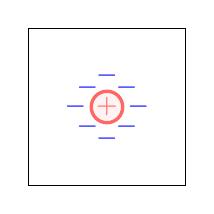
\begin{tikzpicture}
    \draw[] (0, 0) -- (0, 2) -- (2, 2) -- (2, 0) -- cycle;
    \draw[color=red!60, fill=red!5, very thick] (1, 1) circle (.2cm) node {+};
    \node[blue] at (1, 1.4) {$-$};
    \node[blue] at (1.25, 1.25) {$-$};
    \node[blue] at (1.4, 1) {$-$};
    \node[blue] at (1.25, 0.75) {$-$};
    \node[blue] at (1, 0.6) {$-$};
    \node[blue] at (0.75, 0.75) {$-$};
    \node[blue] at (0.6, 1) {$-$};
    \node[blue] at (0.75, 1.25) {$-$};
\end{tikzpicture}
\end{document}